%%%%%%%%%%%%%%%%%%%%%%%%%%%%%%%%%%%%%%%%%
% kaobook
% LaTeX Template
% Version 1.3 (December 9, 2021)
%
% This template originates from:
% https://www.LaTeXTemplates.com
%
% For the latest template development version and to make contributions:
% https://github.com/fmarotta/kaobook
%
% Authors:
% Federico Marotta (federicomarotta@mail.com)
% Based on the doctoral thesis of Ken Arroyo Ohori (https://3d.bk.tudelft.nl/ken/en)
% and on the Tufte-LaTeX class.
% Modified for LaTeX Templates by Vel (vel@latextemplates.com)
%
% License:
% CC0 1.0 Universal (see included MANIFEST.md file)
%
%%%%%%%%%%%%%%%%%%%%%%%%%%%%%%%%%%%%%%%%%

%----------------------------------------------------------------------------------------
%	PACKAGES AND OTHER DOCUMENT CONFIGURATIONS
%----------------------------------------------------------------------------------------

\PassOptionsToPackage{noautomatic}{imakeidx} % Disable automatic indexing
\documentclass[
	b5paper, % Page size
	fontsize=10pt, % Base font size
	twoside=true, % Use different layouts for even and odd pages (in particular, if twoside=true, the margin column will be always on the outside)
	%open=any, % If twoside=true, uncomment this to force new chapters to start on any page, not only on right (odd) pages
	%chapterentrydots=true, % Uncomment to output dots from the chapter name to the page number in the table of contents
	numbers=noenddot, % Comment to output dots after chapter numbers; the most common values for this option are: enddot, noenddot and auto (see the KOMAScript documentation for an in-depth explanation)
]{kaobook}

\usepackage[disablepatch=caption]{tocbasic}

\usepackage{fontspec}
\usepackage{xeCJK}
\xeCJKsetup{space=true}

\setmainfont{NotoSerifCJKkr-Regular.otf}[
  Path=fonts/noto/,
  BoldFont=NotoSerifCJKkr-Bold.otf,
  ItalicFont=NotoSerifCJKkr-Regular.otf,
  ItalicFeatures={FakeSlant=0.2},
  BoldItalicFont=NotoSerifCJKkr-Bold.otf,
  BoldItalicFeatures={FakeSlant=0.2}
]
\setCJKmainfont{NotoSerifCJKkr-Regular.otf}[
  Path=fonts/noto/,
  BoldFont=NotoSerifCJKkr-Bold.otf,
  ItalicFont=NotoSerifCJKkr-Regular.otf,
  ItalicFeatures={FakeSlant=0.2},
  BoldItalicFont=NotoSerifCJKkr-Bold.otf,
  BoldItalicFeatures={FakeSlant=0.2}
]
\setCJKsansfont{NotoSansCJKkr-Regular.otf}[
  Path=fonts/noto/,
  BoldFont=NotoSansCJKkr-Bold.otf,
  ItalicFont=NotoSansCJKkr-Regular.otf,
  ItalicFeatures={FakeSlant=0.2},
  BoldItalicFont=NotoSansCJKkr-Bold.otf,
  BoldItalicFeatures={FakeSlant=0.2}
]
\setCJKmonofont{NotoSansCJKkr-Regular.otf}[
  Path=fonts/noto/,
  BoldFont=NotoSansCJKkr-Bold.otf,
  ItalicFont=NotoSansCJKkr-Regular.otf,
  ItalicFeatures={FakeSlant=0.2},
  BoldItalicFont=NotoSansCJKkr-Bold.otf,
  BoldItalicFeatures={FakeSlant=0.2}
]
%     \newfontfamily\hangulfont{NotoSerifCJKkr-Regular.otf}[
%       Path=fonts/noto/,
%       BoldFont=NotoSerifCJKkr-Bold.otf,
%       ItalicFont=NotoSerifCJKkr-Regular.otf,
%       ItalicFeatures={FakeSlant=0.2},
%       BoldItalicFont=NotoSerifCJKkr-Bold.otf,
%       BoldItalicFeatures={FakeSlant=0.2}
%     ]
%     \newfontfamily\hangulfontsf{NotoSansCJKkr-Regular.otf}[
%       Path=fonts/noto/,
%       BoldFont=NotoSansCJKkr-Bold.otf,
%       ItalicFont=NotoSansCJKkr-Regular.otf,
%       ItalicFeatures={FakeSlant=0.2},
%       BoldItalicFont=NotoSansCJKkr-Bold.otf,
%       BoldItalicFeatures={FakeSlant=0.2}
%     ]
%     \newfontfamily\hangulfonttt{NotoSansCJKkr-Regular.otf}[
%       Path=fonts/noto/,
%       BoldFont=NotoSansCJKkr-Bold.otf,
%       ItalicFont=NotoSansCJKkr-Regular.otf,
%       ItalicFeatures={FakeSlant=0.2},
%       BoldItalicFont=NotoSansCJKkr-Bold.otf,
%       BoldItalicFeatures={FakeSlant=0.2}
%     ]    
\usepackage{setspace}
    
\usepackage{tikz}
\usetikzlibrary{arrows.meta, positioning, calc}

% Choose the language
\ifxetexorluatex
% 	\usepackage{polyglossia}
% 	\setmainlanguage{korean}
%     \setotherlanguage{english}
    \usepackage[english]{babel}
\else
	\usepackage[english]{babel} % Load characters and hyphenation
\fi

\usepackage[
  backend=biber,
  style=ieee,
  language=auto,
  autolang=other,
  backref=true
]{kaobiblio}

\usepackage[english=british]{csquotes}	% English quotes

% Load packages for testing
\usepackage{blindtext}
%\usepackage{showframe} % Uncomment to show boxes around the text area, margin, header and footer
%\usepackage{showlabels} % Uncomment to output the content of \label commands to the document where they are used

% Load the bibliography package
\usepackage{kaobiblio}
\addbibresource{main.bib} % Bibliography file

% Load mathematical packages for theorems and related environments
\usepackage[framed=true]{kaotheorems}

% Load the package for hyperreferences
\usepackage{kaorefs}

\graphicspath{{examples/documentation/images/}{images/}} % Paths in which to look for images

\makeindex[columns=3, title=색인, intoc] % Make LaTeX produce the files required to compile the index

\makeglossaries % Make LaTeX produce the files required to compile the glossary
\input{glossary.tex} % Include the glossary definitions

\makenomenclature % Make LaTeX produce the files required to compile the nomenclature

% Reset sidenote counter at chapters
%\counterwithin*{sidenote}{chapter}

%----------------------------------------------------------------------------------------
\DeclareLanguageMapping{korean}{english}
\DeclareQuoteAlias{british}{korean}

\addto\captionsenglish{
	\renewcommand{\contentsname}{목차}
	\renewcommand{\listfigurename}{그림 목차}
	\renewcommand{\listtablename}{표 목차}
	\renewcommand{\figurename}{그림}
	\renewcommand{\tablename}{표}
	\renewcommand{\bibname}{참고 문헌}
}

\begin{document}

%----------------------------------------------------------------------------------------
%	BOOK INFORMATION
%----------------------------------------------------------------------------------------

\titlehead{데이터 기반 마케팅을 위한 \texttt{온톨로지} 가이드}
\subject{Data-Driven Marketing}

%\title[Example and documentation of the {\normalfont\texttt{kaobook}} class]{Example and documentation \\ of the {\normalfont\texttt{kaobook}} class}
\title[마케팅을 이해하는 {\texttt{온톨로지}}]{마케팅을 이해하는 {\texttt{온톨로지}}}
\subtitle{논리로 설계하는 관계의 기술}

\author[김정석, Ph.D.]{김정석, Ph.D.\thanks{Ontology \& Neuro-Symbolic AI Researcher}}

\date{\today}

\publishers{지그재그}

%----------------------------------------------------------------------------------------

\frontmatter % Denotes the start of the pre-document content, uses roman numerals

%----------------------------------------------------------------------------------------
%	OPENING PAGE
%----------------------------------------------------------------------------------------

%\makeatletter
%\extratitle{
%	% In the title page, the title is vspaced by 9.5\baselineskip
%	\vspace*{9\baselineskip}
%	\vspace*{\parskip}
%	\begin{center}
%		% In the title page, \huge is set after the komafont for title
%		\usekomafont{title}\huge\@title
%	\end{center}
%}
%\makeatother

%----------------------------------------------------------------------------------------
%	COPYRIGHT PAGE
%----------------------------------------------------------------------------------------

\makeatletter
\uppertitleback{\@titlehead} % Header

\lowertitleback{
 \textbf{저작권} \\
	\copyright\ 2025 \@author \\
 이 책의 저작권은 저자에게 있습니다. 저작권법에 의해 보호를 받는 저작물이므로 저자와 출판사의 문서에 의한 허락 없이 무단 전재와 복제를 금합니다.
	
	\medskip
	
 \textbf{발행} \\
	2025년 12월, \@publishers 발행
}
\makeatother

%----------------------------------------------------------------------------------------
%	DEDICATION
%----------------------------------------------------------------------------------------

\dedication{
	\vspace*{0.15\textheight} % Visually balanced vertical spacing
	\begin{center}
		스스로의 길을 찾기 위해 끊임없이 질문을 던지고,\\
		비록 잠시 멈추더라도 끝내 앞으로 나아가려는\\
		모든 분들께 이 책을 바칩니다.\\[2em]
		
		여러분의 걸음은 언제나 깊은 의미를 지니며,\\
		그 여정은 생각보다 훨씬 더 먼 곳에 닿을 것입니다.
	\end{center}
}

%----------------------------------------------------------------------------------------
%	OUTPUT TITLE PAGE AND PREVIOUS
%----------------------------------------------------------------------------------------

% Note that \maketitle outputs the pages before here

\maketitle
 
%----------------------------------------------------------------------------------------
%	PREFACE
%----------------------------------------------------------------------------------------

\chapter*{서문}
\addcontentsline{toc}{chapter}{서문} % Add the preface to the table of contents as a chapter
\setstretch{1.6}
마케팅과 온톨로지는 모두 {\normalfont\texttt{관계}}라는 단어를 사용한다. 그러나 같은 단어를 사용한다고 해서 이들이 같은 의미를 담고 있는 것은 아니다. 두 영역에서 관계라는 단어는 서로 완전히 다른 개념적
틀을 가지고 사용된다. 이 점을 서문의 시작에서 분명하게 하고자 한다.

먼저 \texttt{마케팅에서의 관계(relationship)}는 주로 사람과 사람, 혹은 고객과 브랜드 사이의 심리적이고 정서적인 유대감을 의미한다. 이 관계는 신뢰, 충성도, 애착, 만족감과 같은 감성적이며 주
관적인 연결성을 나타낸다. 마케팅은 바로 이 유대감을 형성하고 유지하며 강화하는 활동으로, 최근의 마케팅 연구들은 이를 \enquote{관계의 설계}\parencite{gummesson2008}로 표현하기도 한다.
반면, \texttt{온톨로지에서의 관계(relation)}는 주관적이거나 감성적이지 않다. 온톨로지에서의 관계는 명확히 정의된 \texttt{엔티티(entity)}들 사이의 구조적이고 객관적인 연결이다. 특정 \texttt{주체(subject)}와 \texttt{객체(object)}가 어떤 \texttt{의미적 관계(predicate)}로 연결되어 있는지 논리적으로 명시하는 것이 온톨로지적 관계이다.
예를 들어,\enquote{고객이 제품을 구매하다}, 혹은 \enquote{사용자가 서비스를 이용하다}와 같은 관계가 온톨로지적 의미의 관계이다.

이 책은 마케팅을 온톨로지적 방법으로 분석하고 활용하는 것을 목적으로 한다. 그렇기에 두 영역에서 사용되는 용어와 개념을 혼동하지 않도록 초반부터 명확히 구분하는 것이 중요하다. 마케팅적 관계
의 감성적이고 심리적인 요소는, 온톨로지에서 사용되는 객관적이고 구조적인 관계로 명료하게 재구성되어야 한다. 이를 통해 비로소 마케팅을 온톨로지적으로 명확하게 분석하고, 설계하고, 실행할 수 있다.

\begin{flushright}
	\textit{저자}
\end{flushright}

\setstretch{1.2}


%----------------------------------------------------------------------------------------
%	TABLE OF CONTENTS & LIST OF FIGURES/TABLES
%----------------------------------------------------------------------------------------

\begingroup % Local scope for the following commands

% Define the style for the TOC, LOF, and LOT
%\setstretch{1} % Uncomment to modify line spacing in the ToC
%\hypersetup{linkcolor=blue} % Uncomment to set the colour of links in the ToC
\setlength{\textheight}{230\hscale} % Manually adjust the height of the ToC pages

% Turn on compatibility mode for the etoc package
\etocclasstocstyle % "toc display" as if etoc was not loaded
\etocstandardlines % "toc lines" as if etoc was not loaded

\tableofcontents % Output the table of contents

\listoffigures % Output the list of figures

% Comment both of the following lines to have the LOF and the LOT on different pages
\let\cleardoublepage\bigskip
\let\clearpage\bigskip

\listoftables % Output the list of tables

\endgroup

%----------------------------------------------------------------------------------------
%	MAIN BODY
%----------------------------------------------------------------------------------------

\mainmatter % Denotes the start of the main document content, resets page numbering and uses arabic numbers
\setchapterstyle{kao} % Choose the default chapter heading style

\pagelayout{wide} % No margins
\addpart{마케팅, 판단의 기술}
%\pagelayout{wide} % No margins

\pagelayout{margin}
\setstretch{1.8}
\setchapterpreamble[u]{\margintoc}
\chapter{메시지 과잉의 시대}
\labch{messageoverflow}

\section{관계의 언어}

마케팅은 결국, 복잡한 선택의 순간마다 가장 적절한 판단을 내리는 기술이다\cite{kotler2021marketing, schwartz2004paradox, thaler2008nudge, court2009consumer, kahneman2011thinking}. 고객을 누구로 정의할 것인지, 어떤 가치를 전달할 것인지, 어느 경로를 통해 연결할 것 인지를 끊임없이 결정해야 한다. 결국 \index{마케팅}마케팅이란, 수많은 가능성들 사이에서 하나의 방향을 선택하는 판단의 기술이자 구조의 예술이다.


\begin{figure}[h] 
\caption{고객-브랜드-제품}
\labfig{customer-brand-product}
\centering
\begin{tikzpicture}[
    entity/.style={circle, draw=black, thick, minimum size=1.8cm, font=\bfseries, align=center},
    rel/.style={->, thick, >=Latex},
    curved/.style={rel, bend left=25},
    curved_right/.style={rel, bend left=-20},
    curvedback/.style={rel, bend right=25}
]
% 원 위에 엔티티 배치
\node[entity] (customer) at (90:3cm) {고객};
\node[entity] (brand)    at (200:3.5cm) {브랜드};
\node[entity] (product)  at (340:3.5cm) {제품};

% 관계선 (곡선)
\draw[curved] (customer) to node[right=4pt] {\small 구매함} (product);
\draw[curved] (product) to node[below left=4pt] {\small 대표함} (brand);
\draw[curved_right] (brand)   to node[above right=4pt] {\small 제공함} (product);
\draw[curved] (brand)   to node[above left=4pt] {\small 소통} (customer);
\draw[curved_right] (customer) to node[below right=2pt] {\small 신뢰함} (brand);
\draw[curved_right] (product) to node[below left=4pt] {\small 만족함} (customer);


\end{tikzpicture}
\end{figure}

판단은 고립된 정보로부터 만들어지지 않는다.
우리가 어떤 대상을 이해하고 선택하며 행동으로 옮기는 과정에는,
언제나 그 대상이 다른 요소들과 맺고 있는 관계에 대한 인식이 작동한다.
무엇이 중요하고, 어떤 흐름이 존재하는가를 알기 위해서는 반드시 관계를 정의해야 한다.
\index{판단}판단은 관계를 전제로 하는 기술이며, \index{관계}관계는 구조를 전제로 한다.

마케팅에서의 판단도 마찬가지다.
\enquote{무엇을 만들 것인가}, \enquote{누구에게 제공할 것인가}, \enquote{어떤 방식으로 전달할 것인가}라는 질문은 모두 관계를 기반으로 움직인다.
이때 말하는 관계는 단지 고객과 브랜드 사이의 감정적 연결만을 의미하지 않는다.
고객, 브랜드, 제품이라는 세 개의 핵심 주체는 마케팅 활동의 중심에 자리 잡고 있으며 이들 간의 관계는 단순한 1:1 연결이 아니라, \reffig{customer-brand-product}처럼 상호작용의 흐름 속에서 의미가 교차되고, 기대가 형성되며, 가치가 이동하는 구조를 가진다.

\textbf{고객과 브랜드의 관계}

브랜드는 고객에게 끊임없이 말을 건다. 광고를 통해, 메시지를 통해, 심지어는 제품의 디자인이나 포장 하나하나를 통해 브랜드는 자신이 어떤 존재인지 설명하고자 한다. 이에 대해 고객은 그 말을 듣고 판단한다. 신뢰할 수 있을지, 기대에 부합할지, 그리고 앞으로 계속 관계를 이어갈 수 있을지를 말이다.

고객은 브랜드를 신뢰하고, 브랜드는 고객에게 소통한다. 이 양방향의 관계는 시간이 쌓이며 강화되기도 하고, 때로는 약해지기도 한다. 마케팅은 바로 이 균형을 다루는 기술이다.


\textbf{제품과 문제 상황의 관계}

제품은 그 자체로 존재하지 않는다. 항상 문제 상황을 해결하기 위해 설계된 수단이다. 갈증을 해소하고, 지루함을 달래며, 불편을 줄인다. 고객은 어떤 문제 상황에서 제품을 찾고, 그 해결 능력을 통해 제품을 평가한다.

\reffig{customer-brand-product} 다이어그램에서는 이 관계가 직접 그려져 있지는 않지만, 고객이 제품을 \enquote{구매하고}, 제품이 고객을 \enquote{만족시키는} 흐름 속에서 문제 해결의 내재된 구조가 드러난다.
제품이 문제를 제대로 해결하지 못했다면 만족은 없을 것이며, 반복 구매도 기대할 수 없다.

\textbf{\index{채널}채널과 \index{접점}접점의 관계}

마케팅에서 채널은 고객에게 메시지를 전달하고, 제품을 유통하며, 브랜드를 노출시키는 전달 경로를 의미한다. 이는 TV 광고, 소셜 미디어, 매장, 앱, 디지털 사이니지처럼 다양하며, 물리적일 수도 있고 디지털일 수도 있다. 접점(touchpoint)은 이 채널을 통해 고객과 브랜드, 제품이 실제로 만나는 순간을 뜻한다. 
다시 말해, 채널은 메시지의 길이라면, 접점은 경험이 발생하는 장면이다. 고객은 이 접점에서 브랜드를 느끼고, 제품을 보고, 자신의 필요를 해석한다. 접점은 따라서 단순한 노출이 아니라 의미와 판단이 발생하는 인터페이스\sidenote{여기서 말하는 인터페이스는 접점과 혼동해서는 안 된다. 접점이 고객 경험이 실제로 벌어지는 하나의 장면이라면, 인터페이스는 그 장면 안에서 고객이 직접 마주하고 조작하며 해석하는 작동 면을 뜻한다. 이는 포장을 손에 쥐고 읽는 동작처럼 물리적일 수도 있고, 디지털 사이니지의 화면 구성이나 앱의 UI처럼 디지털일 수도 있다. 하나의 접점 안에는 여러 인터페이스가 존재할 수 있으며, 고객은 이 인터페이스를 통해 메시지를 이해하고 제품을 평가하며 판단을 내린다. 즉, 인터페이스는 접점의 품질을 결정하는 \texttt{구체적 상호작용의 단위}다.}다.

예를 들어, 고객이 카페에서 대기 중일 때 눈앞의 디지털 사이니지를 통해 한 브랜드의 메시지를 접하고, 매장 진열대에 놓인 제품을 집어 들고, 그 기능과 포장을 살펴본다고 하자. 이 모든 일은 하나의 마케팅 접점 안에서 일어난다. 그리고 이 장면은 바로 채널이 제공한 \index{경험의 장}경험의 장이다.

\textbf{시간과 반복의 관계}

\index{신뢰}신뢰는 단지 고객이 브랜드를 한 번 보고 느낀 감정이 아니다. 그것은 시간에 따라 누적된 일관된 경험과 반복적인 상호작용을 통해 천천히 구축되는 구조다.
고객은 브랜드가 제시한 메시지를 접하고, 제품을 사용하며, 그 결과에 만족하거나 실망한다. 이 일련의 과정이 반복되면서 브랜드에 대한 감정은 굳어지고, 기대치는 명확해지며, 결국 특정 브랜드를 선택하는 행동의 패턴이 만들어진다.
이때 중요한 점은, 시간과 반복은 고객–브랜드–제품의 각 개체\sidenote{고객과 제품은 \index{객체}객체(\index{object}object)로 정의할 수 있으나, 브랜드의 경우에는 객체보다 넓은 범위의 독립적으로 존재하는 개념을 지칭하므로, 이를 포괄하는 \texttt{\index{개체}개체(\index{entity}entity)}로 정의한다.}를 따로 관통하지 않고, 이 셋을 하나의 폐쇄 루프처럼 연결하면서 작동한다는 것이다. 즉, 고객은 브랜드로부터 제안받은 제품을 반복적으로 사용하고, 그 경험이 다시 브랜드에 대한 신뢰로 연결되며, 이는 다음 구매로 이어지는 선순환 구조를 만든다.

\reffig{customer-brand-product} 다이어그램에서 \texttt{신뢰함}과 \texttt{만족함}이라는 관계는 각각 개별적인 방향성을 가지지만, 실제 마케팅 현실에서 시간과 반복은 이들 관계를 넘나들며, 총체적인 관계의 강화와 변화를 유도하는 리듬처럼 작동한다.마케팅이 이 리듬을 이해하고 조율한다면, 고객과 브랜드 사이의 연결은 한 번의 선택이 아니라 습관이 된 선택, 즉 \index{충성도}\enquote{충성도}가 될 수 있다.

\textbf{고객 내부 요소 간의 관계}

고객의 행동은 표면만 봐서는 설명되지 않는다. 우리가 보는 것은 브랜드에 대한 신뢰, 제품에 대한 구매, 사용 후의 만족과 같은 행동의 결과일 뿐이다. 그러나 그 결정 뒤에는 언제나 욕구와 감정, 기대와 기억 같은 내부 요소들이 서로 영향을 주며 작동하고 있다.이 내면의 구조는 지금까지 다루었던 다이어그램 속에는 직접적으로 표현되지 않는다.

고객은 외부 자극에 반응하는 단순한 객체가 아니라 스스로 판단하고 행동을 선택하는 의사 결정의 주체이기 때문에, 고객 내부 요소 간의 상호작용은 일련의 활동을 분석하는 핵심 축 중 하나가 된다.

\begin{figure}[h]
\centering
\begin{tikzpicture}[
    entity/.style={circle, draw=black, thick, minimum size=2cm, font=\bfseries, align=center},
    innernode/.style={font=\small, align=center},
    hidden/.style={font=\scriptsize, gray},
    rel/.style={->, thick, >=Latex},
    curved/.style={rel, bend left=25},
    curved_right/.style={rel, bend left=-20},
    curvedback/.style={rel, bend right=25}
]

% 엔티티 노드 배치
\node[entity] (customer) at (90:5cm) {고객};
\node[entity] (brand)    at (200:4cm) {브랜드};
\node[entity] (product)  at (340:4cm) {제품};

% 고객 내부 요소
\node[innernode] (desire) at ($(customer)+(130:2cm)$) {\scriptsize 욕구};
\node[innernode] (emotion) at ($(customer)+(50:2cm)$) {\scriptsize 감정};
\node[innernode] (expectation) at ($(customer)+(10:2cm)$) {\scriptsize 기대};
\node[innernode] (memory) at ($(customer)+(180:2cm)$) {\scriptsize 기억};

% 제품 내부 요소
\node[innernode] (function) at ($(product)+(20:2cm)$) {\scriptsize 기능};
\node[innernode] (design) at ($(product)+(-5:2cm)$) {\scriptsize 디자인};

% 브랜드 요소
\node[innernode] (message) at ($(brand)+(140:2cm)$) {\scriptsize 메시지};
\node[innernode] (symbol) at ($(brand)+(180:2cm)$) {\scriptsize 상징성};

% 접점 노드
\node[entity, minimum size=1.5cm, font=\small] (touchpoint) at (90:1cm) {\scriptsize 접점};

% 채널 노드 (이너노드로 표현)
\node[hidden] (channel_app) at ($(touchpoint)+(10:2cm)$) {앱};
\node[hidden] (channel_store) at ($(touchpoint)+(120:2cm)$) {매장};
\node[hidden] (channel_signage) at ($(touchpoint)+(240:2cm)$) {사이니지};

% 관계선
\draw[curved] (customer) to node[right=4pt] {\small 구매함} (product);
\draw[curved] (product) to node[below left=4pt] {\small 대표함} (brand);
\draw[curved_right] (brand)   to node[above right=4pt] {\small 제공함} (product);
\draw[curved] (brand)   to node[above left=4pt] {\small 소통} (customer);
\draw[curved_right] (customer) to node[below right=4pt] {\small 신뢰함} (brand);
\draw[curved_right] (product) to node[below left=4pt] {\small 만족함} (customer);

% 고객과 접점, 제품과 접점 연결
\draw[rel, dashed] (customer) -- (touchpoint);
\draw[rel, dashed] (product) -- (touchpoint);
\draw[rel, dashed] (brand) -- (touchpoint);


% 채널 → 접점 연결
\draw[dashed, gray] (channel_app) -- (touchpoint);
\draw[dashed, gray] (channel_store) -- (touchpoint);
\draw[dashed, gray] (channel_signage) -- (touchpoint);

% 내면 요소와 고객 연결
\foreach \x in {desire, emotion, expectation, memory} {
    \draw[dashed, gray] (\x) -- (customer);
}

% 제품 내부 요소와 제품 연결
\foreach \x in {function, design} {
    \draw[dashed, gray] (\x) -- (product);
}

\foreach \x in {message, symbol} {
    \draw[dashed, gray] (\x) -- (brand);
}

\end{tikzpicture}
\caption{관계의 확장}
\end{figure}

즉, 고객이 브랜드를 \texttt{신뢰}하고, 제품을 \texttt{구매}하며, 결과에 \texttt{만족}하는 일련의 흐름은 모두 눈에 보이는 외부적 상호작용이다. 반면에 \texttt{왜} 고객이 신뢰했는지, \texttt{무엇}이 그를 만족시켰는지, \texttt{어떤} 감정이 반복 구매로 이어졌는지는 고객 내면의 일이다. 이 보이지 않는 관계를 다룰 수 있어야 비로소 마케팅은 설득을 넘어 이해의 단계에 도달하게 되는 것이다. 

그리고 이 구조를 다루기 위해서는 데이터에 대한 단순한 분석을 넘어 그 관계와 상황에 대한 맥락을 이해해야만 한다.
\section{관계의 목적}
앞에서 우리는 고객, 브랜드, 제품, 채널, 시간, 그리고 고객의 내면 요소까지 포함한 관계의 구조를 살펴보았다. 이제 질문은 구조가 아니라 \texttt{목적}이다. 이 모든 관계를 왜 설계하려 하는가, 그리고 그 관계는 무엇을 위해 존재해야 하는가. 목적이 불명확한 관계 설계는 대개 \enquote{더 많이, 더 자주 말하자}로 수렴한다. 그러나 메시지 과잉의 시대에 그것은 설득이 아니라 노이즈의 축적이 된다.

관계의 목적은 하나로 고정되지 않는다. 같은 관계라도 \texttt{제품 중심}, \texttt{고객 중심}, \texttt{브랜드 중심}으로 관점을 옮기면 목적의 정의가 달라지고, 그에 따라 측정 지표와 실행 전략도 달라진다. 아래는 세 관점을 명확히 분리해 정리한 관계의 목적이다.

\textbf{제품 중심의 관계 목적: 약속을 증명하는 구조}

제품 관점에서 관계는 감정적 유대의 장식이 아니라, \texttt{약속을 검증하는 실험 환경}이다. 고객이 브랜드를 평가하는 최종 근거는 콘텐츠나 캠페인이 아니라 제품 경험이며, 관계는 이 경험이 반복적으로 누적될 수 있도록 경로를 설계한다. 따라서 제품 중심의 관계 목적은 다음 세 가지로 정리된다.

\begin{description}
  \item[관계의 실체화]
  신뢰나 호감 같은 추상적 유대는 제품 경험을 통해서만 실체를 얻는다. 제품은 \enquote{브랜드의 약속이 고객의 현실에서 작동하는지}를 판명하는 장(場)이며, 관계는 그 검증이 일어나는 조건을 안정적으로 만든다.

  \item[문제 해결의 일관성]
  고객이 구매하는 것은 제품이 아니라 \texttt{문제 해결의 가능성}이다. 관계의 목적은 제품이 고객의 결핍과 불편을 해소하고, 기대(Expectation)를 만족(Satisfaction)으로 전환하는 경험을 지속적으로 제공하도록 만드는 데 있다.

  \item[판단 비용 절감의 패턴 형성]
  만족스러운 제품 경험이 축적되면 고객의 인지 속에 \enquote{이 브랜드/이 제품군은 안전하다}는 \index{휴리스틱}휴리스틱이 만들어진다.\sidenote{휴리스틱은 심리학, 인지과학에서 자주 쓰이는 말로 모든 정보를 완벽하게 따져보지 못할 때, 경험과 직관을 활용해 \enquote{그럴듯한} 결론에 빠르게 도달하게 해주는 판단의 요령을 뜻한다.} 제품 중심 관계의 목적은 이 패턴을 형성해 향후 구매에서 비교, 탐색, 의심에 드는 \texttt{판단 비용}을 낮추는 것이다.
\end{description}

제품 중심에서 관계의 목적은 브랜드의 \enquote{약속}을 고객 경험 속 \enquote{현실}로 반복 증명하는 구조를 만드는 일이다.

\textbf{고객 중심의 관계 목적: 선택을 돕는 환경}

고객 관점에서 관계는 브랜드의 메시지를 받아들이는 통로가 아니라, \texttt{삶의 과업을 더 쉽게 수행하게 하는 환경}이다. 고객은 언제나 시간, 주의, 예산이 부족하고 정보는 과잉이다. 관계는 이 제약 속에서 고객이 더 적은 노력으로 더 좋은 결정을 내리도록 만든다. 고객 중심의 관계 목적은 다음과 같다.

\begin{description}
  \item[인지 부담과 탐색 비용의 최소화]
  고객은 모든 대안을 충분히 비교할 수 없다. 관계는 필요한 정보가 필요한 시점에 도달하도록 하여 탐색 비용을 낮추고, \enquote{알아보기}에 쓰는 시간을 \enquote{사용하기}로 전환시킨다.

  \item[맥락 기반 선택 지원]
  같은 제품이라도 고객의 상황(시간, 장소, 동기, 제약)에 따라 최적 선택은 달라진다. 관계의 목적은 고객의 맥락을 이해하고, 그 맥락에 맞는 옵션을 좁혀 제시해 \texttt{선택의 난이도}를 낮추는 것이다.

  \item[안전감과 통제감의 제공]
  관계가 성립했다는 것은 고객이 \enquote{실패해도 감당 가능한 선택}을 할 수 있다는 뜻이기도 하다. 고객 중심의 관계 목적은 사후 지원, 교환/환불, 사용 가이드, 책임의 명료화를 통해 구매의 불확실성과 위험 인식을 낮추는 데 있다.
\end{description}

고객 중심에서 관계의 목적은 고객의 제약을 전제로 \texttt{불확실성을 낮추고 선택을 돕는 의사결정 환경}을 제공하는 것이다.

\textbf{브랜드 중심의 관계 목적: 최적화하는 판단 체계}

브랜드 관점에서 관계는 \texttt{설득의 감정적 언어}가 아니라, 한정된 자원을 어디에 어떻게 배분할지 결정하는 \texttt{운영의 기준}이다. 브랜드는 시장의 모든 사람에게 동일한 강도로 다가갈 수 없고, 따라서 관계는 \enquote{누구에게 집중할 것인가}를 정의한다. 브랜드 중심의 관계 목적은 다음과 같이 정리된다.

\begin{description}
  \item[우선순위의 설정과 자원 배분]
  관계는 잠재 고객을 동일한 집단으로 보지 않게 만든다. 상호 이해와 신뢰가 누적된 고객군은 더 낮은 설득 비용으로 더 높은 반응을 기대할 수 있으며, 브랜드는 관계 강도에 따라 예산, 채널, 메시지의 밀도를 재배치한다.

  \item[설득 비용의 절감과 효율의 상승]
  관계가 형성된 고객에게는 설명과 설득의 비용(\index{CAC}CAC\sidenote{CAC(Customer Ac\-qui\-si\-tion Cost)는 신규 고객 한 명을 확보하기 위해 지출하는 비용(마케팅비, 영업비 등)의 총합을 의미한다. 관계가 깊어질수록 기존 고객의 재구매율이 높아져 전체적인 CAC는 낮아지는 효과가 있다.})이 줄어든다. 브랜드 중심의 목적은 \texttt{동일한 성과를 더 적은 비용으로} 내는 구조를 만드는 것이며, 이는 반복 구매, 재방문, 전환율, 추천의 형태로 나타난다.

  \item[의미의 일관성과 정체성 유지]
  브랜드는 상황마다 다른 말을 하면 단기 반응을 얻을 수는 있어도 장기 신뢰를 잃는다. 관계의 목적은 제품/채널/메시지가 서로 충돌하지 않도록 정체성을 유지하고, 고객의 기대를 안정적으로 관리하는 데 있다.
\end{description}

브랜드 중심에서 관계의 목적은 \texttt{누구에게 무엇을 얼마나 투자할지 결정하는 판단 체계}를 만들고, 그 결과로 설득 비용과 운영 비용을 동시에 낮추는 것이다.

\textbf{정리: 하나의 관계, 세 개의 목적}

같은 관계라도 관점에 따라 목적은 다르게 정의된다. 제품 중심은 \enquote{약속의 증명}, 고객 중심은 \enquote{선택의 지원}, 브랜드 중심은 \enquote{자원 배분의 최적화}에 초점이 있다. 이 세 목적이 동시에 성립할 때, 관계는 단순한 커뮤니케이션이 아니라 \index{판단 비용}\texttt{판단 비용을 낮추는 시스템}이 된다.

\section{신뢰의 조건}

% Content to be added

\section{투명성의 기반}

앞서 신뢰를 \enquote{판단 비용을 낮추는 조건}으로 정의했다면, 투명성은 그 조건을 충족시키기 위한 가장 구체적인 실천 원칙이다. 흔히 투명성을 \enquote{모든 것을 숨기지 않고 공개하는 것}으로 오해하기 쉽다. 하지만 마케팅의 관점에서 정보의 무차별적인 공개는 오히려 노이즈가 된다.\sidenote{신뢰를 구축하는 투명성의 핵심은 양(Quantity)이 아니라, 고객이 필요할 때 사실을 확인할 수 있는가 하는 \texttt{\enquote{검증 가능한 정보에 대한 접근성}}에 있다.}

고객이 브랜드의 메시지를 의심하는 이유는 정보가 부족해서가 아니라, 그 정보가 브랜드의 이익을 위해 편향되었을 것이라 가정하기 때문이다\cite{friestad1994persuasion}. 따라서 투명성의 본질은 고객이 브랜드의 주장을 스스로 검증할 수 있는 수단을 제공함으로써, 의심을 해소하는 비용을 브랜드가 대신 지불하는 데 있다. 이를 위해 투명성은 다음 두 가지 핵심 요소를 기반으로 설계되어야 한다.

\textbf{정보의 완전성}

\index{정보의 완전성}정보의 완전성(Completeness)이란 고객이 의사결정을 내리는 데 필수적인 정보가 누락되지 않았음을 의미한다. 이는 단순히 많은 정보를 나열하는 것이 아니라, 고객에게 불리할 수 있는 정보(단점, 부작용, 추가 비용, 공정상의 한계 등)까지도 감추지 않고 제공하는 것을 뜻한다.

경제학의 \index{정보 비대칭}정보 비대칭(Information Asymmetry) 이론은 판매자가 구매자보다 더 많은 정보를 가질 때 시장의 신뢰가 무너지고 거래 비용이 증가함을 설명한다\cite{akerlof1970market}. 마케팅에서의 투명성은 이 비대칭을 의도적으로 해소하는 행위다. 브랜드가 먼저 약점을 공개하면 고객은 숨겨진 위험을 찾기 위해 방어적인 태도를 취할 필요가 없어진다. 즉, 정보의 완전성은 고객이 \enquote{내가 모르는 함정이 있을지 모른다}는 불안감을 내려놓게 만드는 장치다.

\textbf{맥락의 공유}

\index{사실}\index{Fact}사실(Fact)\sidenote{\texttt{사실(Fact)}이란 가격 인상, 배송 지연, 기능 변경 등 겉으로 드러난 현상 그 자체를 의미한다. 이는 \texttt{결과값(Result)}일 뿐, 그 결과가 발생하게 된 의도나 배경을 포함하지 않는 데이터다.}만으로는 충분하지 않다. 같은 가격 인상이라도 \enquote{원자재 가격 상승으로 인해 불가피했다}는 맥락이 공유된 경우와, 아무런 설명 없이 가격이 오른 경우는 고객에게 전혀 다르게 받아들여진다. 맥락의 공유(Context Sharing)는 결과값(What)뿐만 아니라, 그 결과가 나오게 된 과정과 기준(Why/How)을 설명하는 것이다\cite{buell2019operational}.

\begin{itemize}
    \item \texttt{기준의 공개}: 교환이나 환불 정책, 멤버십 등급 산정 등 브랜드가 고객을 대우하는 기준이 명확하고 일관되게 공개되어야 한다.
    \item \texttt{과정의 공개}: 제품이 만들어지는 과정, 서비스가 지연된 이유, 문제가 발생했을 때의 대처 과정 등을 공유함으로써 고객을 관찰자가 아닌 참여자로 만든다.
\end{itemize}

맥락이 공유되지 않은 정보는 오해를 낳기 쉽다. 반면, 의사결정의 배경과 기준을 투명하게 밝히면 고객은 비록 그 결과가 자신에게 다소 불편하더라도 브랜드의 의도를 악의적으로 해석하지 않게 된다. 

\vspace{1em}

\begin{figure}[h]
\centering
\begin{tikzpicture}[
    block/.style={rectangle, draw=black, thick, rounded corners, minimum width=3cm, minimum height=1.2cm, align=center, font=\bfseries},
    subtext/.style={font=\small\normalfont, color=gray},
    arrow/.style={->, thick, >=Latex}
]

% Nodes
\node[block] (complete) at (-3.5, 2) {정보의 완전성\\\footnotesize(판단의 재료)};
\node[block] (context) at (3.5, 2) {맥락의 공유\\\footnotesize(해석의 기준)};
\node[block, minimum width=4cm] (verify) at (0, 0) {검증 가능한 정보\\\footnotesize(접근성)};
\node[block, draw=none, fill=gray!10] (trust) at (0, -2) {신뢰\\\footnotesize(의심 비용 제거)};

% Paths
\draw[arrow] (complete) -- (verify);
\draw[arrow] (context) -- (verify);
\draw[arrow] (verify) -- (trust);

\end{tikzpicture}
\caption{투명성의 기반 구조}
\labfig{foundation-of-transparency}
\end{figure}

\vspace{1em}

결론적으로 투명성의 기반은 \enquote{모든 것을 보여주는 것}이 아니라, \enquote{의심할 필요가 없도록 만드는 것}이다. \texttt{정보의 완전성}을 통해 판단의 재료를 숨김없이 제공하고, \texttt{맥락의 공유}를 통해 그 재료를 해석하는 기준까지 제공할 때, 고객은 브랜드를 검증의 대상이 아닌 신뢰의 파트너로 인식하기 시작한다. 이는 곧 마케팅 비용을 줄이고 관계의 수명을 늘리는 가장 경제적인 전략이 된다.


\setchapterpreamble[u]{\margintoc}
\chapter{판단의 기준}
\labch{criteriaofjudgement}

\section{직관의 한계}

\section{맥락의 파편화}

\section{구조적 해결책}



\pagelayout{wide} % No margins
\addpart{온톨로지, 논리의 설계}
\pagelayout{margin} % No margins

\setstretch{1.8}
\setchapterpreamble[u]{\margintoc}
\chapter{온톨로지의 본질}
\labch{originofontology}

\section{의미의 합의}

우리가 사용하는 언어는 근본적으로 불완전하다. 같은 단어를 사용한다고 해서 같은 대상을 지칭하는 것은 아니다. 2장에서 살펴보았듯이, \enquote{충성도}나 \enquote{가치} 같은 핵심적인 비즈니스 용어조차 개인의 경험과 직관에 따라 전혀 다른 의미로 해석되곤 한다.\sidenote{이러한 언어적 모호성은 소통의 비용을 증가시키고, 판단의 일관성을 무너뜨리는 주된 원인이 된다.}

\index{온톨로지}\texttt{온톨로지(Ontology)}의 본질은 이러한 모호함을 걷어내기 위한 \enquote{의미의 합의} 과정에 있다. 기술적인 정의는 잠시 배제하고 본질적인 관점에서 설명하자면, 온톨로지는 \enquote{우리가 무엇에 대해 이야기하고 있는가}를 명확히 정의하고, 그 정의를 지키기로 한 구성원\sidenote{여기서 구성원이란 사람뿐만 아니라, 시스템을 구성하는 모든 개체를 의미한다. 즉, 데이터를 생성하고 소비하는 소프트웨어, 그리고 이를 학습하는 인공지능(AI)까지를 포함하는 포괄적인 개념이다.} 간의 \texttt{약속(Promise)}이다.

\vspace{1em}
\noindent\textbf{언어의 불확실성 (Uncertainty of Language)}

일상 대화에서 약간의 오해는 유연하게 넘어갈 수 있다. 하지만 비즈니스, 특히 데이터와 시스템이 개입되는 환경에서 모호한 정의는 치명적인 결과를 초래한다.

예를 들어, A라는 시스템이 정의하는 \enquote{신규 고객}은 \enquote{이번 달에 처음으로 회원 가입한 사람}일 수 있다. 반면, B라는 시스템이 처리하는 \enquote{신규 고객}은 \enquote{이번 달에 첫 구매를 발생시킨 사람}일 수 있다. 이 두 정의가 혼재된 상태에서 \enquote{신규 고객 유치 전략}을 데이터를 통해 분석하려 한다면, 결과는 왜곡될 수밖에 없다. 서로 다른 대상을 같은 이름으로 부르고 있기 때문이다.

이러한 불확실성은 단순히 용어집(Glossary)\sidenote{용어집이란 특정 도메인에서 사용되는 용어와 그 정의를 모아둔 문서를 말한다. 이는 구성원들이 동일한 단어를 동일한 의미로 이해하도록 돕는 1차적인 기준점 역할을 수행하여 의사소통의 혼선을 줄이는 데 기여한다.}을 만든다고 해결되지 않는다. 용어집은 단어의 뜻을 나열할 뿐, 그 단어들이 서로 어떤 관계를 맺고 있는지, 어떤 맥락에서 유효한지까지는 강제하지 못하기 때문이다. 따라서 우리에게는 단순한 사전적 정의를 넘어, 대상을 바라보는 관점을 일치시키는 더 강력한 도구가 필요하다.

\vspace{1em}
\noindent\textbf{존재에 대한 규정 (Defining Existence)}

온톨로지라는 단어는 원래 \enquote{존재론}을 뜻하는 철학 용어에서 유래했다. 즉, \enquote{무엇이 존재하는가}를 규명하는 학문이다. 마케팅 시스템을 구축하는 과정에서도 이 질문은 가장 먼저 던져져야 한다.

\textit{우리 비즈니스 세계에 \texttt{무엇이 존재하는가?}}

이 질문에 답하는 것이 온톨로지 설계의 시작이다. 우리는 \enquote{고객}이 존재한다고 합의한다. \enquote{상품}이 존재하고, \enquote{구매}라는 행위가 존재한다고 합의한다. 너무나 당연해 보이는 이 과정이 중요한 이유는, 우리가 합의하여 정의하지 않은 대상은 시스템 안에서 존재할 수 없기 때문이다.

명확하게 정의된 존재만이 데이터로 포착될 수 있고, 논리의 재료로 사용될 수 있다. 온톨로지는 이처럼 모호한 현실 세계의 대상들을 명확한 경계를 가진 \enquote{개념}으로 확정 짓는 작업이다.

\vspace{1em}
\noindent\textbf{약속으로서의 구조 (Structure as a Promise)}

이렇게 합의된 정의는 단순한 텍스트로 남아서는 안 된다. 그것은 시스템 전체가 반드시 지켜야 할 \texttt{약속}이 되어야 한다.

\textit{우리가 \texttt{구매}라고 말할 때는, 반드시 \texttt{결제 완료} 상태이면서 \texttt{환불되지 않은} 거래만을 의미하기로 약속한다.}

이 약속이 지켜질 때, 비로소 데이터는 신뢰를 얻는다. 온톨로지는 이 약속을 시스템의 언어, 즉 구조적인 형태로 기록한 것이다. 누군가의 머릿속에만 있는 암묵적인 규칙이 아니라, 시스템이 검증하고 강제할 수 있는 형태로 명문화된 약속이다.

결국 온톨로지를 구축한다는 것은, 내재화된 직관적인 언어를 걷어내고, 모두가 동의하고 검증할 수 있는 \enquote{약속의 언어}를 만드는 과정이다. 이 약속이 견고할수록, 우리는 불필요한 해석의 논쟁 없이 데이터가 가리키는 현상 그 자체에 집중할 수 있게 된다.

\section{관계의 구조화}

의미의 모호함을 걷어내기 위해 \enquote{약속}이 필요하다는 점은 자명하다. 그렇다면 이 약속을 어떻게 시스템에 기록하고 강제할 수 있을까? 

단순한 단어의 정의만으로는 부족하다. 약속을 구체적이고 명확하게 표현하기 위해서는, 단어와 단어 사이의 관계를 규정하는 \enquote{문법(Grammar)}이 필요하다. 우리가 정의한 개념들이 비즈니스의 \enquote{어휘(Vocabulary)}라면, 온톨로지는 이 어휘들을 엮어 흔들리지 않는 약속의 문장을 만드는 \enquote{문법}이다.

\vspace{1em}
\noindent\textbf{단어에서 문장으로 (From Words to Sentences)}

\enquote{쿠키(Cookie)}라는 단어를 생각해보자. 이 단어 하나만으로는 그것이 \enquote{먹는 과자}인지, \enquote{웹 브라우저의 데이터}인지 알 수 없다. 맥락이 부재하기 때문이다. 하지만 다음과 같이 문장으로 표현하면 의미는 명확해진다.

\begin{itemize}
    \item \texttt{Cookie}는 \texttt{사용자 정보}를 \texttt{저장한다(Stores)}.
    \item \texttt{Cookie}는 \texttt{초콜릿}을 \texttt{함유한다(Contains)}.
\end{itemize}

첫 번째 문장에서의 Cookie는 IT 기술 용어이고, 두 번째 문장에서는 간식이다. 이처럼 단어의 진짜 의미는 독립적으로 존재하지 않으며, 다른 단어와의 \texttt{관계} 속에서 비로소 결정된다. 온톨로지는 바로 이 \enquote{관계}를 구조적으로 정의하는 체계다.

\vspace{1em}
\noindent\textbf{의미의 최소 단위: 주어-서술어-목적어}

온톨로지에서 모든 정보는 가장 단순하고 명확한 구조인 \enquote{주어(Subject) - 서술어(Predicate) - 목적어(Object)}의 형태로 기록된다. 이 세 가지 요소가 모여 하나의 단위를 구성하기 때문에, 이를 \texttt{트리플(Triple)}이라 부른다.

\begin{itemize}
    \item \textbf{주어(Subject)}: 행위의 주체 또는 설명의 대상 (예: 고객)
    \item \textbf{서술어(Predicate)}: 주어와 목적어 사이의 관계 (예: ~을 구매하다)
    \item \textbf{목적어(Object)}: 행위의 대상 또는 속성값 (예: 상품)
\end{itemize}

우리가 흔히 사용하는 \enquote{고객이 상품을 구매했다}라는 문장도 이 구조를 따른다.

\begin{center}
    \texttt{고객(Customer)} $\xrightarrow{\text{구매하다(Buys)}}$ \texttt{상품(Product)}
\end{center}

이처럼 세상의 모든 복잡한 현상을 이 세 가지 요소를 사용해 \enquote{누가(Who), 무엇을(What), 어떻게(How)} 연결되는지로 분해하여 기록하는 것이 온톨로지 모델링의 핵심이다.

\begin{figure}[ht]
    \centering
    \includegraphics[width=0.9\textwidth]{figures/ch03/ontology_graph_visualization.png}
    \caption[복잡하게 연결된 온톨로지 그래프]{복잡하게 연결된 온톨로지 그래프의 예시. 단어(Node)와 관계(Edge)가 거미줄처럼 연결되어 거대한 의미의 그물망을 형성한다.}
    \label{fig:ontology-graph}
\end{figure}

\vspace{1em}
\noindent\textbf{구조화의 힘 (Power of Structure)}

왜 굳이 이렇게 딱딱한 구조로 정보를 기록해야 할까? 그 이유는 \texttt{기계가 이해할 수 있는 형태}이기 때문이다.

사람은 \enquote{김철수 고객님이 어제 A 상품을 샀어요}라는 문장을 읽고 바로 이해할 수 있다. 하지만 컴퓨터 시스템에게 이 문장은 그저 텍스트 데이터일 뿐이다. 반면, 이를 \texttt{김철수(Subject)} - \texttt{구매하다(Predicate)} - \texttt{A상품(Object)}이라는 구조로 전달하면, 시스템은 비로소 \enquote{구매}라는 관계를 인식하고 처리할 수 있게 된다.

또한 이 구조는 확장이 용이하다. \texttt{A상품}이 어떤 \texttt{카테고리}에 속하는지, 그 카테고리는 어떤 \texttt{상위 분류}에 속하는지를 계속해서 꼬리에 꼬리를 물고 연결할 수 있다.

\begin{center}
    \texttt{고객} $\to$ \texttt{구매} $\to$ \texttt{상품} $\to$ \texttt{소속} $\to$ \texttt{카테고리}
\end{center}

이렇게 연결된 의미의 그물망을 따라가면, \enquote{특정 카테고리를 선호하는 고객}을 찾아내거나, \enquote{함께 구매될 가능성이 높은 상품}을 추천하는 등의 고차원적인 추론이 가능해진다. 이것이 바로 온톨로지가 단순한 데이터 저장소를 넘어, \enquote{지능형 시스템}의 기반이 되는 이유다.


\section{논리의 검증}


\setchapterpreamble[u]{\margintoc}
\chapter{모델링의 실제}
\labch{practicalmodeling}



\section{욕구의 계층화}

이제 우리는 이론적 논의를 넘어, 마케팅의 실체적 대상들을 모델링할 단계에 이르렀다. 온톨로지를 설계한다는 것은 결국 \enquote{무엇이 존재하는가}를 정의하고, 그 존재들이 \enquote{어떤 관계를 맺는가}를 규명하는 작업이다.

마케팅의 세계를 구성하는 세 가지 핵심 주체는 \texttt{고객(Customer)}, \texttt{제품(Product)}, 그리고 \texttt{브랜드(Brand)}다. 이들이 서로 관계를 맺는 원동력은 무엇일까? 바로 각 주체가 가진 고유한 \enquote{욕구(Needs)}다. 인간에게 매슬로우의 욕구 위계가 있듯이\sidenote{매슬로우(Abraham Maslow)의 욕구 위계 이론(1943)은 인간의 동기가 하위 단계(생리적 욕구)에서 상위 단계(자아실현)로 발전한다고 설명한다. 마케팅에서는 이를 차용하여 고객이 제품을 통해 얻고자 하는 혜택의 단계를 설명하는 데 자주 사용한다.}, 제품과 브랜드에도 시장에서 생존하고 성장하기 위한 그들만의 욕구 위계가 존재한다.

이 섹션에서는 각 주체의 욕구를 구조화하여, 온톨로지 모델링의 기초 뼈대를 세워보자.


\vspace{1em}
\noindent\textbf{고객의 욕구 위계}

고객이 제품을 구매하는 행위는 단순히 물건을 소유하기 위함이 아니다. 그 이면에는 해결하고자 하는 문제나 도달하고자 하는 상태가 있다. 수단-목표 사슬 이론(Means-End Chain Theory)은 이를 잘 설명한다.

\begin{itemize}
    \item \textsf{1단계: 기능적 욕구 (Functional Needs)} \\
    가장 밑바닥에는 \enquote{결핍의 해소}가 있다. 배가 고프면 음식이 필요하고, 이동해야 하면 탈것이 필요하다. 이는 제품의 \enquote{속성(Attribute)}과 직접적으로 연결된다.
    \item \textsf{2단계: 정서적 욕구 (Emotional Needs)} \\
    기능이 충족되면 감정이 개입한다. 단순히 이동하는 것을 넘어, \enquote{편안함}이나 \enquote{안전함}, 혹은 \enquote{운전의 즐거움}을 원한다. 이는 제품 사용의 \enquote{결과(Consequence)}로 얻어지는 혜택이다.
    \item \textsf{3단계: 가치적 욕구 (Life Needs)} \\
    최상위에는 고객의 \enquote{자아(Self)}가 있다. 친환경 제품을 쓰며 \enquote{의식 있는 소비자}가 되고 싶거나, 명품을 통해 \enquote{성공한 사람}으로 인정받고 싶은 욕구다. 이는 고객의 \enquote{가치(Value)}를 실현한다.
\end{itemize}

\begin{figure}[h!]
    \centering
    \begin{tikzpicture}[scale=0.85, transform shape]
        % Define Triangle vertices (Standard size is sufficient now)
        \coordinate (A) at (0, 4.5);
        \coordinate (B) at (-4, 0);
        \coordinate (C) at (4, 0);

        % Draw Pyramid Outline
        \draw [thick] (B) -- (C) -- (A) -- cycle;

        % Draw Horizontal Lines for Levels
        \coordinate (L1_Left) at (-2.66, 1.5);
        \coordinate (L1_Right) at (2.66, 1.5);
        \coordinate (L2_Left) at (-1.33, 3);
        \coordinate (L2_Right) at (1.33, 3);

        \draw [thick] (L1_Left) -- (L1_Right);
        \draw [thick] (L2_Left) -- (L2_Right);

        % Add Level Labels (Inside - Simple Terms)
        \node [align=center, font=\bfseries] at (0, 0.75) {속성\\(Attributes)};
        \node [align=center, font=\bfseries] at (0, 2.25) {결과\\(Consequences)};
        \node [align=center, font=\bfseries] at (0, 3.60) {가치\\(Values)};

        % Add Meaning Labels (Right Side - Detailed Needs)
        \node [right, align=left, font=\small] at (4.2, 0.75) { $\leftarrow$ \textbf{1단계: 기능적 욕구} \\ \hspace{1.2em} (Functional Needs)};
        \node [right, align=left, font=\small] at (4.2, 2.25) { $\leftarrow$ \textbf{2단계: 정서적 욕구} \\ \hspace{1.2em} (Emotional Needs)};
        \node [right, align=left, font=\small] at (4.2, 3.60) { $\leftarrow$ \textbf{3단계: 가치적 욕구} \\ \hspace{1.2em} (Life Needs)};
    \end{tikzpicture}
    \caption[고객 욕구 위계]{고객 욕구의 위계 구조}
    \labfig{customer-needs-pyramid}
\end{figure}


\vspace{1em}
\noindent\textbf{제품의 욕구 위계}

제품을 하나의 개체로 본다면, 시장에서 살아남기 위해 무엇이 필요할까?

\begin{itemize}
    \item \textsf{1단계: 존재의 욕구 (Existence)} \\
    가장 기본은 \enquote{가용성(Availability)}이다. 고객이 살 수 있는 곳에 있어야 하고, 적절한 가격표가 붙어 있어야 한다. 재고가 없거나 가격이 책정되지 않은 제품은 시장에 \enquote{존재}하지 않는 것과 같다.
    \item \textsf{2단계: 기능의 욕구 (Functionality)} \\
    존재한다면 제 구실을 해야 한다. 스펙(Spec)대로 작동해야 하며, 약속한 성능을 제공해야 한다. 이것이 충족되지 않으면 제품은 즉시 도태된다.
    \item \textsf{3단계: 편의의 욕구 (Usability)} \\
    기능이 아무리 좋아도 쓰기 불편하면 선택받기 힘들다. 접근하기 쉽고, 사용하기 쉬워야 한다\sidenote{사용자 경험(User Experience, UX)은 사용자가 제품, 시스템, 서비스를 이용하면서 느끼는 지각과 반응, 행동 등 총체적인 경험을 의미한다. 단순히 기능적인 편리함을 넘어, 감정적인 만족, 가치, 심미적인 즐거움까지 포함하는 포괄적인 개념이다.}.
    \item \textsf{4단계: 매력의 욕구 (Desirability)} \\
    마지막 단계는 \enquote{갖고 싶게 만드는 것}이다. 디자인, 패키징, 그리고 제품이 가진 스토리가 여기에 해당한다.
\end{itemize}


\vspace{1em}
\noindent\textbf{브랜드의 욕구 위계}

브랜드는 제품에 의미를 부여하여, 고객의 마음속에 자리 잡기를 원한다. 켈러(Kevin Lane Keller)의 브랜드 자산 모델(CBBE\sidenote{고객 기반 브랜드 자산(Customer-Based Brand Equity, CBBE) 모델은 브랜드의 가치가 고객의 마음속에 형성된 지식에 의해 결정된다는 이론이다. 강력한 브랜드를 구축하기 위해 브랜드 정체성(Identify)에서 시작해 의미(Meaning), 반응(Response)을 거쳐 최종적으로 공명(Resonance)에 이르는 4단계의 피라미드 구조를 제시한다.})은 브랜드가 성장하는 과정을 명확한 위계로 보여준다\cite{keller2013strategic}.

\begin{itemize}
    \item \textsf{1단계: 정체성의 욕구 (Identity)} \\
    \enquote{나는 누구인가?} 브랜드는 먼저 고객에게 인식되어야 한다. 이를 브랜드 인지도(Salience)라 한다. 고객이 브랜드를 떠올릴 수 없다면 관계는 시작될 수 없다.
    \item \textsf{2단계: 의미의 욕구 (Meaning)} \\
    \enquote{나는 무엇인가?} 인지된 브랜드는 고유한 이미지를 가져야 한다. 탁월한 성능(Performance)이든, 독보적인 이미지(Imagery)든 차별화된 연상 작용을 만들어내야 한다.
    \item \textsf{3단계: 반응의 욕구 (Response)} \\
    \enquote{나에 대해 어떻게 생각하는가?} 고객의 판단(Judgments)과 느낌(Feelings)을 이끌어내야 한다. 신뢰감, 우월감, 혹은 따뜻함과 같은 긍정적 반응이 필요하다.
    \item \textsf{4단계: 관계의 욕구 (Resonance)} \\
    \enquote{나와 당신은 어떤 사이인가?} 최상위 단계는 고객과의 공명(Resonance)이다. 단순한 구매를 넘어 충성도를 가지고 적극적으로 옹호하는 단계다.
\end{itemize}

\begin{figure}[h!]
    \centering
    \begin{tikzpicture}[
        scale=0.82, transform shape,
        node distance=1.0cm and 3.5cm,
        subject/.style={rectangle, draw=blue!60, thick, rounded corners, minimum width=3.0cm, minimum height=0.9cm, align=center, fill=white, font=\ttfamily},
        object/.style={rectangle, draw=red!60, thick, rounded corners, minimum width=3.0cm, minimum height=0.9cm, align=center, fill=white, font=\ttfamily},
        predicate/.style={->, very thick, >=stealth, color=black},
        label/.style={font=\ttfamily\footnotesize, color=black, anchor=west}
    ]
        % Right Column: Objects (Provider Offerings) - Bottom Up
        \node[object] (Obj_Func) {기능/품질\\(Functionality)};
        \node[object, above=1.0cm of Obj_Func] (Obj_Use) {사용성/UX\\(Usability)};
        \node[object, above=1.0cm of Obj_Use] (Obj_Mean) {의미/이미지\\(Meaning)};
        \node[object, above=1.0cm of Obj_Mean] (Obj_Reso) {관계/공명\\(Resonance)};

        % Internal Evolution Arrows (Solid for clarity)
        \draw[->, black!80, thick] (Obj_Func) -- (Obj_Use);
        \draw[->, black!80, thick] (Obj_Use) -- (Obj_Mean);
        \draw[->, black!80, thick] (Obj_Mean) -- (Obj_Reso);
        
        % Right Side Labels (Moved further right to avoid box border)
        \coordinate (RightAlign) at ($(Obj_Func.east) + (0.6, 0)$);
        
        \node[label] at (Obj_Func -| RightAlign) {Product};
        \node[label] at (Obj_Use -| RightAlign) {Product};
        \node[label] at (Obj_Mean -| RightAlign) {Brand};
        \node[label] at (Obj_Reso -| RightAlign) {Brand};


        % Left Column: Subjects (Customer Needs)
        % Position relative to Objects
        \node[subject, left=3.5cm of Obj_Use] (Sub_Func) {기능적 욕구\\(Functional)};
        \node[subject] at (Sub_Func |- Obj_Mean) (Sub_Emot) {정서적 욕구\\(Emotional)};
        \node[subject] at (Sub_Func |- Obj_Reso) (Sub_Life) {가치적 욕구\\(Life)};

        % Predicates (Mapping Arrows)
        % Functional -> Usability
        \draw[predicate] (Sub_Func) -- node[midway, fill=white, font=\ttfamily\footnotesize] {require} (Obj_Use);
        
        % Emotional -> Meaning
        \draw[predicate] (Sub_Emot) -- node[midway, fill=white, font=\ttfamily\footnotesize] {seek} (Obj_Mean);
        
        % Life -> Resonance
        \draw[predicate] (Sub_Life) -- node[midway, fill=white, font=\ttfamily\footnotesize] {realize} (Obj_Reso);

        % Background Frames for Context
        % Increased inner sep to ensure arrows and nodes have clearance
        \begin{scope}[on background layer]
             \node[fit=(Sub_Life)(Sub_Func), draw=blue!30, dashed, rounded corners, inner sep=0.4cm, label=above:\textbf{\textsf{Subject (Customer Requirements)}}] {};
             \node[fit=(Obj_Reso)(Obj_Func), draw=red!30, dashed, rounded corners, inner sep=0.4cm, label=above:\textbf{\textsf{Object (Marketer Offerings)}}] {};
        \end{scope}

    \end{tikzpicture}
    \caption[온톨로지 SPO 매핑]{욕구(Subject)와 제공가치(Object)의 온톨로지 매핑}
    \labfig{needs-ontology-mapping}
\end{figure}

이처럼 세 주체는 각자의 욕구 위계를 가지고 있다. 마케팅 온톨로지는 바로 이 욕구들이 서로 어떻게 맞물리는지를 정의하는 거대한 지도로 기능한다. 결국 욕구의 계층화란 \textbf{속성을 식별하고, 그 속성들 간에 어떤 관계를 갖는지 규칙을 정해주는 것}을 의미한다. 고객의 \textit{기능적 욕구}가 제품의 \textit{사용성/UX}와 만나고, \textit{정서적 욕구}가 브랜드의 \textit{의미/이미지}와 만나며, 최종적으로 \textit{가치적 욕구}가 브랜드의 \textit{공명}과 만나는 지점을 정확히 연결하는 것이 바로 모델링의 본질이다.

\section{행동의 인과성}

\section{시간의 축적}



\pagelayout{wide} % No margins
\addpart{경험, 구조의 확장}
\pagelayout{margin} % No margins

\setchapterpreamble[u]{\margintoc}
\chapter{일관된 접점의 구현}
\labch{consistenttouchpoint}

\section{데이터의 통합}

\section{여정의 시각화}

데이터는 보이지 않는다. 서버에 쌓이는 로그는 시간, 접속 IP, 행위의 기록(Log)일 뿐, 그 자체로는 아무런 서사도 보여주지 않는다. 앞서 설계한 온톨로지가 \enquote{지식의 지도}라면, 여정의 시각화(Visualization of Journey)는 그 지도 위에서 실제로 움직이는 \texttt{데이터의 흐름(Flow)}을 검증하는 과정이다.

시각화는 단순히 \enquote{결과를 보여주는 보고서}가 아니다. 온톨로지 관점에서 시각화는 \texttt{데이터 로직의 유닛 테스트(Unit Test for Data Logic)}와 같다. 이는 눈에 보이지 않는 데이터의 연결이 논리적으로 타당한지, 끊어진 곳은 없는지, 설계된 인과관계가 실제 데이터로 증명되는지를 확인하는 논리적 검증 수단이다.

\textbf{정적 스냅샷에서 동적 시퀀스로}

데이터베이스(DB)의 테이블은 \texttt{스냅샷(Snapshot)}이다. \enquote{특정 고객이 특정 시점에 상품을 구매했다}는 사실은 테이블의 한 행(Row)으로 기록된다. 하지만 이것만으로는 데이터 간의 인과관계를 설명할 수 없다. 온톨로지 기반의 시각화는 이 정적인 스냅샷들을 \texttt{시간의 축} 위에서 연결하여 하나의 \texttt{시퀀스(Sequence)}로 변환하는 작업이다.

\begin{itemize}
    \item \texttt{기존의 테이블 뷰}: 사용자(User), 주문(Order), 로그(Log) 테이블이 물리적으로 분리되어 있다. \enquote{누가(Who)}와 \enquote{무엇을(What)}은 존재하지만, 이들이 필연적으로 연결되는지는 알 수 없다.
    \item \texttt{온톨로지 뷰}: \enquote{검색(Search) $\xrightarrow{cause}$ 상품 조회(View) $\xrightarrow{cause}$ 장바구니 담기(Add-to-Cart) $\xrightarrow{cause}$ 구매(Purchase)}라는 데이터의 인과적 흐름이 명시적인 화살표(Edge)로 시각화된다.
\end{itemize}

\begin{figure}[ht]
    \centering
    \resizebox{\linewidth}{!}{
    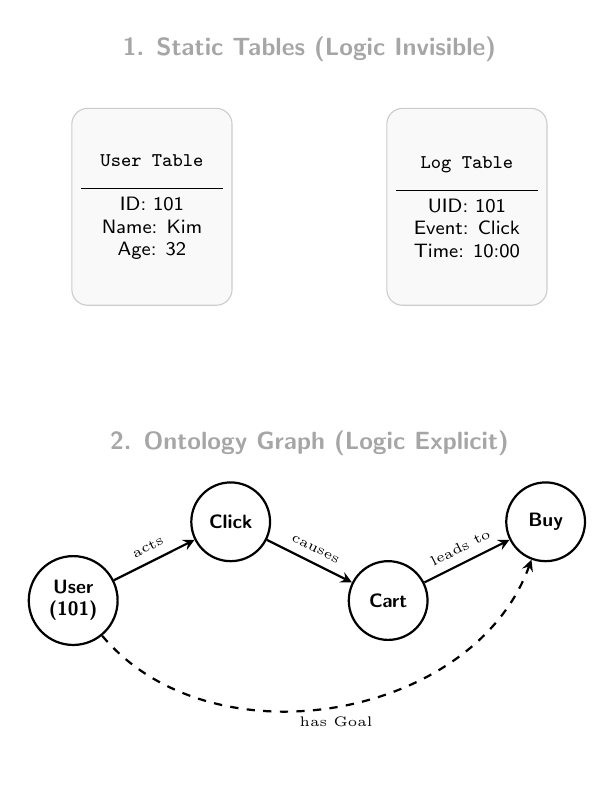
\begin{tikzpicture}[
        node distance=1.5cm,
        table/.style={
            rectangle, 
            draw=gray!40, 
            fill=gray!5, 
            rounded corners=2mm, 
            minimum width=2cm, 
            minimum height=2.5cm, 
            align=center, 
            font=\sffamily\scriptsize
        },
        graphnode/.style={
            circle, 
            draw=black, 
            fill=white, 
            thick, 
            minimum size=1cm, 
            align=center, 
            font=\sffamily\bfseries\scriptsize
        },
        arrow/.style={
            ->, 
            >=stealth, 
            thick, 
            draw=black
        },
        label/.style={
            font=\sffamily\bfseries\small, 
            text=gray!70
        }
    ]

    % --- Part 1: Relational Tables (Static) ---
    \node[label] at (0, 0.5) {1. Static Tables (Logic Invisible)};
    
    \node[table] (user) at (-2, -1.5) {
        \texttt{User Table}\\
        \rule{1.8cm}{0.4pt}\\
        ID: 101\\
        Name: Kim\\
        Age: 32
    };
    
    \node[table] (log) at (2, -1.5) {
        \texttt{Log Table}\\
        \rule{1.8cm}{0.4pt}\\
        UID: 101\\
        Event: Click\\
        Time: 10:00
    };
    
    % --- Part 2: Ontology Graph (Dynamic) ---
    \node[label] at (0, -4.5) {2. Ontology Graph (Logic Explicit)};
    
    \node[graphnode] (u) at (-3, -6.5) {User\\(101)};
    \node[graphnode] (e1) at (-1, -5.5) {Click};
    \node[graphnode] (e2) at (1, -6.5) {Cart};
    \node[graphnode] (e3) at (3, -5.5) {Buy};
    
    % Relationships
    \draw[arrow] (u) -- node[above, sloped, font=\tiny] {acts} (e1);
    \draw[arrow] (e1) -- node[above, sloped, font=\tiny] {causes} (e2);
    \draw[arrow] (e2) -- node[above, sloped, font=\tiny] {leads to} (e3);
    \draw[arrow, dashed, bend right=60] (u) to node[below, font=\tiny] {has Goal} (e3);

    \end{tikzpicture}
    }
    \caption[데이터의 관점 변화: 정적 테이블에서 동적 여정으로]{데이터의 관점 변화: 정적 테이블에서 동적 여정으로. 테이블 구조에서는 알 수 없는 인과관계가 온톨로지 그래프에서는 명시적인 화살표(Edge)로 드러난다.}
    \labfig{table_vs_graph}
\end{figure}

이러한 시각화는 단순히 \enquote{구매가 발생했다}는 결과뿐만 아니라, 그 결과에 도달하기까지의 과정을 \texttt{동적(Dynamic)}으로 보여준다. 만약 시각화된 여정에서 \enquote{장바구니 담기}와 \enquote{구매} 사이의 화살표가 빈번하게 끊어져 있다면, 그것은 단순한 이탈이 아니라 시스템 내 데이터 흐름의 단절을 의미한다.

\textbf{논리적 정합성의 검증}

데이터를 시각화한다는 것은 곧 \texttt{데이터 연결(Edge)의 진실성}을 확인하는 과정이다. \enquote{데이터 기반 의사결정}이 유효하려면, 그 기반이 되는 데이터의 연결 구조가 참(True)이어야 한다.

온톨로지로 시각화된 여정 지도는 전체 데이터 시스템에 대한 \texttt{단일한 논리적 뷰(Unified Logical View)}를 제공한다. \enquote{캠페인 반응 데이터}와 \enquote{구매 전환 데이터}는 별개의 사일로(Silo)에 존재하는 것이 아니라, 하나의 긴 인과 사슬(Causal Chain) 속에서 연결되어야만 한다.

이 과정에서 검증해야 할 핵심 질문은 \enquote{논리적으로 연결되어 있는가?}이다. 시각화 도구 위에서 데이터의 흐름이 끊김 없이 이어진다면, 온톨로지 모델링은 유효한 것이다. 반대로 여정이 끊겨서 보인다면, 그것은 데이터가 파편화되어 있다는 증거다. 결국 시각화는 데이터 통합의 완전성을 증명하는 성적표이자, 데이터 품질을 관리하는 모니터링 수단이 된다.

모든 데이터는 연결되어야 비로소 정보가 되고, 흐름이 되어야 통찰이 된다. 여정의 시각화는 그 흐름을 드러내어, 데이터가 단순한 적재물이 아니라 논리적인 서사를 가진 구조임을 증명한다.

\section{맥락의 최적화}


\setchapterpreamble[u]{\margintoc}
\chapter{관계 설계자의 미래}
\labch{futureofontologist}

\section{인공지능과 협업}

우리가 지금까지 온톨로지를 다뤄온 이유는 단 하나다. 복잡하게 얽힌 고객의 데이터를 이해하고, 그 안에서 의미 있는 관계를 찾아내기 위해서다. 
데이터는 넘쳐나지만 정작 고객은 \enquote{나를 이해하지 못하는 브랜드}에 피로감을 느낀다. 이 간극을 메우기 위해서는 데이터를 쌓는 것을 넘어, 데이터를 \texttt{연결하는 구조}가 필요하다.

바로 이 지점에서 새로운 역할이 요구된다. 단순히 도구를 다루는 기술자가 아니라, 브랜드와 고객 사이의 관계가 어떻게 형성되어야 하는지 그 논리적 밑그림을 그리는 사람, 바로 \texttt{관계 설계자(Relationship Architect)}다.

기존의 관계 마케팅(Relationship Marketing)이 고객과의 장기적 유대감을 강조하는 \enquote{철학}이었다면, 관계 설계자는 그 철학을 데이터와 기술로 구현하는 \enquote{공학자}다.\sidenote{크리스티안 그뢴로스(Christian Grönroos)\cite{gronroos1994marketing}나 에버트 구메손(Evert Gummesson)\cite{gummesson2008}과 같은 학자들은 마케팅의 본질이 '관계'에 있다고 주창했다. 관계 설계자는 이 이론적 토대 위에, 온톨로지라는 공학적 방법론을 더해 추상적인 관계를 구체적인 시스템의 언어로 구현하는 사람을 의미한다.} 우리는 이 새로운 직함을 통해 마케팅의 영역을 감각의 세계에서 논리의 세계로 확장한다.

\textbf{관계 설계자와 온톨로지스트의 결합}

관계 설계자는 마케팅이라는 도메인 안에서 탄생한 개념이다. 하지만 그 본질을 들여다보면 필연적으로 온톨로지스트가 될 수밖에 없다. 왜냐하면 현대의 마케팅에서 \enquote{관계를 설계한다}는 것은 곧 \enquote{데이터 간의 관계를 정의한다}는 말과 동의어이기 때문이다.

\enquote{건성 피부인 고객에게 수분 크림을 추천한다}는 마케팅 전략은, 데이터 세계에서는 \texttt{Subject(User:DrySkin)} $\rightarrow$ \texttt{Predicate(needs)} $\rightarrow$ \texttt{Object(Product:Moisturizer)}라는 온톨로지 명제로 변환되어야 한다. 마케터가 자신의 전략을 시스템이 이해할 수 있는 구조로 정의하지 못한다면, 그 전략은 실행될 수 없다. 즉, 마케팅의 의도를 데이터의 구조로 번역하는 능력, 그것이 바로 온톨로지스트로서의 역량이다.

다행스러운 점은, 우리가 컴퓨터 과학자처럼 복잡한 코드나 수식으로 온톨로지의 내부를 깊이 파고들 필요는 없다는 것이다. 이제 우리에게는 그 복잡성을 대신 처리해줄 강력한 파트너, \texttt{인공지능(AI)}이 있기 때문이다. 우리는 AI에게 논리적 설계도만 건네주면 된다.

\textbf{역할의 분담: 계산하는 AI, 설계하는 인간}

이 협업의 구조는 명확하다. 인간은 \enquote{무엇(What)}과 \enquote{왜(Why)}를 정의하고, AI는 \enquote{어떻게(How)}를 실행한다.

\begin{itemize}
    \item \textbf{AI의 역할 (The Engine)}: AI는 인간이 설계한 온톨로지 구조 안에서 방대한 데이터를 실시간으로 처리한다. 수백만 명의 고객이 남기는 파편화된 \texttt{단서(Clues)}를 \texttt{온톨로지 그래프}에 매핑하고, 가장 적합한 경로를 계산하여 즉각적인 \texttt{제안(Offer)}을 실행한다. 이것은 인간의 인지 능력을 넘어서는 \enquote{규모(Scale)}와 \enquote{속도(Speed)}의 영역이다.
    
    \item \textbf{인간의 역할 (The Architect)}: 인간은 시스템이 작동할 \texttt{논리적 기반(Logical Foundation)}을 만든다. \enquote{왜 이 고객에게 이 시점에 이 메시지를 보내야 하는가?}에 대한 인과관계를 설정하고, 시스템이 놓칠 수 있는 윤리적 판단이나 브랜드의 철학을 주입한다. 또한, AI가 내놓은 결과값이 현실 세계의 맥락과 부합하는지 검증하고(Validation), 끊임없이 온톨로지를 수정하고 보완한다.
\end{itemize}

즉, AI는 \enquote{주어진 길을 가장 빠르게 달리는 운전자}라면, 인간은 \enquote{그 길이 어디로 향해야 하는지 정하고 도로를 닦는 설계자}가 된다.

\textbf{운영자에서 설계자로}

과거의 디지털 마케터는 \enquote{운영자(Operator)}에 가까웠다. 광고 입찰가를 조정하고, 타겟팅 옵션을 설정하고, 소재를 교체하는 반복적인 작업이 주를 이뤘다. 하지만 AI가 이 모든 운영 업무를 자동화하는 시대에, 운영자로서의 마케터는 설 자리를 잃어가고 있다.

하지만 \texttt{설계자(Architect)}로서의 마케터는 대체 불가능하다. 어떤 데이터를 수집할 것인지, 그 데이터에 어떤 의미를 부여할 것인지, 그리고 고객과 어떤 관계를 맺고 싶은지에 대한 \enquote{질문}은 오직 인간만이 던질 수 있기 때문이다.

관계 설계자는 도구의 사용법을 익히는 사람이 아니라, 도구가 작동하는 \texttt{원리}를 만드는 사람이다. 마케터가 온톨로지스트가 되어야 하는 이유는, 결국 기술을 지배하는 힘이 코드가 아닌 \enquote{논리}에서 나오기 때문이다. AI 시대, 가장 강력한 경쟁력은 가장 인간적인 \enquote{관계에 대한 통찰}을 구조화하는 능력이다.

\section{초개인화의 완성}

우리는 오랫동안 \index{세그먼테이션}\texttt{세그먼테이션(Segmentation)}이라는 개념\cite{smith1956product}에 의존해왔다.\sidenote{웬델 스미스(Wendell Smith)가 1956년 제안한 시장 세분화 개념은 대량 생산 시대의 공급 과잉을 해결하기 위한 돌파구였다. 하버드 교육대학원의 토드 로즈(Todd Rose) 역시 그의 저서 \textit{평균의 종말(The End of Average)}에서 \enquote{평균적인 인간은 없다}고 단언하며, 집단 기반의 사고방식이 개개인을 설명하는 데 얼마나 취약한지를 증명했다.\cite{rose2016end}} 
20대 여성, 서울 거주자, 구매력이 높은 직장인. 이것은 거대한 시장을 관리 가능한 단위로 쪼개기 위한 효율적인 방법이었지만, 결코 완벽한 방법은 아니었다. 
왜냐하면 \enquote{20대 서울 거주 여성}이라는 집단 안에는 수천 가지의 서로 다른 욕망과 맥락이 혼재되어 있기 때문이다.

진정한 의미의 개인화, 즉 \index{초개인화}\texttt{초개인화(Hyper-Personalization)}는 집단을 나누는 것이 아니라,
집단이라는 개념 자체를 해체하는 것에서 시작된다. 이것은 돈 페퍼스(Don Peppers)가 주창한 \enquote{Segment of One}\cite{peppers1993one}, 
즉 오직 한 사람만을 위한 시장을 만드는 일이다.\sidenote{돈 페퍼스와 마사 로저스(Martha Rogers)는 \textit{일대일 미래(The One to One Future)}에서 시장 점유율(Market Share)이 아닌 고객 점유율(Share of Customer)을 높이는 것이 미래의 경쟁력이라고 역설했다. 초개인화는 이 개념을 기술적으로 완성하는 단계다.} 

\textbf{정적 데이터에서 동적 맥락으로}

기존의 개인화가 \index{정적 데이터}\texttt{정적 데이터(Static Data)}에 기반했다면, 초개인화는 \index{동적 맥락}\texttt{동적 맥락(Dynamic Context)}에 반응한다.
예를 들어보자.

\begin{itemize}
    \item \textbf{기존 개인화}: \enquote{A 고객은 30대 남성이므로 스포츠 용품을 추천한다.} (고정된 속성)
    \item \textbf{초개인화}: \enquote{A 고객이 지금 폭설이 내리는 지역에 있고, 방금 '방수'라는 키워드를 검색했다.} (변화하는 맥락)
\end{itemize}

전자가 \enquote{그 사람이 누구인가(Who)}에 집중한다면, 후자는 \enquote{그 사람이 지금 어떤 상황인가(When \& Where)}와 \enquote{무엇을 원하고 있는가(What \& Why)}를 파악한다. 온톨로지는 이 복잡한 동적 맥락을 실시간으로 해석할 수 있는 구조를 제공한다. \texttt{Snow(Weather)} $\rightarrow$ \texttt{cause(Need)} $\rightarrow$ \texttt{Waterproof(Function)} $\rightarrow$ \texttt{Boots(Product)}라는 인과관계의 사슬이 시스템 내부에서 순식간에 연결되기 때문이다.

\begin{figure}[ht]
    \centering
    \resizebox{\textwidth}{!}{
        \begin{tikzpicture}[
    node distance=2cm, 
    every node/.style={font=\sffamily\small},
    user/.style={circle, draw=black!70, fill=gray!10, thick, minimum size=1.2cm, align=center},
    segment/.style={rectangle, draw=black!60, fill=white, dashed, minimum width=2.5cm, minimum height=3cm, rounded corners},
    context/.style={regular polygon, regular polygon sides=6, draw=teal, fill=teal!10, thick, minimum size=1.2cm, align=center},
    offer/.style={rectangle, draw=black, fill=black!80, text=white, rounded corners, minimum width=2.5cm, minimum height=1cm, align=center},
    arrow/.style={->, >=stealth, thick, color=black!70}
]

% Panel A: Segmentation (Left)
\node[label=above:\textbf{A. Segmentation (Static)}] (labelA) at (0, 4.5) {};

\node[user] (user1) at (0, 0) {User A};
\node[user] (user2) at (-1, -1.5) {User B};
\node[user] (user3) at (1, -1.5) {User C};

% Group Box (Background)
\begin{scope}[on background layer]
    \node[segment, fit=(user1) (user2) (user3), label=below:\texttt{Demographic Group}] (group) {};
\end{scope}

% Offer
\node[offer, above=1.5cm of user1] (offerA) {Offer:\\Generic Coupon};
\draw[arrow] (offerA) -- (group);

% Panel B: Hyper-Personalization (Right)
\node[label=above:\textbf{B. Hyper-Personalization (Dynamic)}] (labelB) at (8, 4.5) {};

\node[user] (userH) at (8, 0) {User A};

% Context Nodes (Adjusted spacing)
\node[context, above left=1.0cm of userH] (ctx1) {Snowing\\(Weather)};
\node[context, above right=1.0cm of userH] (ctx2) {Search:\\Waterproof};
\node[context, below=1.2cm of userH] (ctx3) {Location:\\Ski Resort};

% Ontology Connections
\draw[dashed, color=teal] (ctx1) -- (userH);
\draw[dashed, color=teal] (ctx2) -- (userH);
\draw[dashed, color=teal] (ctx3) -- (userH);

% Perfect Offer
\node[offer, right=2.0cm of userH, fill=teal, text=white] (offerH) {Perfect Offer:\\Waterproof Boots};

% Inference Arrow
\draw[arrow, ultra thick, teal] (userH) -- node[above, font=\footnotesize\bfseries]{Inference} (offerH);

% Separation Line
\draw[thick, dotted] (4, 4.5) -- (4, -3);

\end{tikzpicture}

    }
    \caption[세그먼테이션과 초개인화의 비교]{세그먼테이션과 초개인화의 비교: 정적 집단에서 동적 개인으로의 진화}
    \label{fig:hyper-personalization}
\end{figure}

\textbf{완벽한 제안(The Perfect Offer)}

관계 설계자가 구축한 온톨로지 위에서 AI는 고객의 숨겨진 의도를 읽어낸다. 그리고 가장 적절한 순간(Right Time)에, 가장 적절한 채널(Right Channel)을 통해, 가장 적절한 메시지(Right Message)를 전달한다. 이것이 바로 \index{완벽한 제안}\texttt{완벽한 제안(The Perfect Offer)}이다.

이 수준에 도달하면 마케팅은 더 이상 \enquote{방해(Interruption)}가 아니라 \enquote{도움(Help)}이 된다. 고객은 브랜드가 나에게 무언가를 팔려고 한다는 느낌보다는, 내 문제를 해결해주려 한다는 느낌을 받게 된다. 

초개인화의 완성은 기술의 승리가 아니다. 그것은 브랜드가 고객 한 사람 한 사람을 고유한 인격체로 대우할 수 있게 되었다는, 관계의 승리다. 온톨로지는 그 깊은 이해와 존중을 시스템화하는 언어다.

\section{설계자의 태도}



%\input{chapters/introduction.tex}

%\pagelayout{wide} % No margins
%\addpart{Class Options, Commands and Environments}
%\pagelayout{margin} % Restore margins

%\input{chapters/options.tex}
%\input{chapters/textnotes.tex}
%\input{chapters/figsntabs.tex}
%\input{chapters/references.tex}

%\pagelayout{wide} % No margins
%\addpart{Design and Additional Features}
%\pagelayout{margin} % Restore margins


%\input{chapters/layout.tex}
%\input{chapters/mathematics.tex}

\appendix % From here onwards, chapters are numbered with letters, as is the appendix convention

\pagelayout{wide} % No margins
\addpart{부록}
\pagelayout{margin} % Restore margins

%\input{chapters/appendix.tex}

%----------------------------------------------------------------------------------------

\backmatter % Denotes the end of the main document content
\setchapterstyle{plain} % Output plain chapters from this point onwards

%----------------------------------------------------------------------------------------
%	BIBLIOGRAPHY
%----------------------------------------------------------------------------------------

% The bibliography needs to be compiled with biber using your LaTeX editor, or on the command line with 'biber main' from the template directory

\printbibliography[heading=bibintoc, title=참고 문헌] % Add the bibliography heading to the ToC, set the title of the bibliography

%----------------------------------------------------------------------------------------
%	NOMENCLATURE
%----------------------------------------------------------------------------------------

% The nomenclature needs to be compiled on the command line with 'makeindex main.nlo -s nomencl.ist -o main.nls' from the template directory

%\nomenclature{$c$}{Speed of light in a vacuum inertial frame}
%\nomenclature{$h$}{Planck constant}

%\renewcommand{\nomname}{Notation} % Rename the default 'Nomenclature'
%\renewcommand{\nompreamble}{The next list describes several symbols that will be later used within the body of the document.} % Prepend this text to the nomenclature

%\printnomenclature % Output the nomenclature

%----------------------------------------------------------------------------------------
%	GREEK ALPHABET
% 	Originally from https://gitlab.com/jim.hefferon/linear-algebra
%----------------------------------------------------------------------------------------

%\vspace{1cm}

%----------------------------------------------------------------------------------------
%	GLOSSARY
%----------------------------------------------------------------------------------------

% The glossary needs to be compiled on the command line with 'makeglossaries main' from the template directory

%\setglossarystyle{listgroup} % Set the style of the glossary (see https://en.wikibooks.org/wiki/LaTeX/Glossary for a reference)
%\printglossary[title=Special Terms, toctitle=List of Terms] % Output the glossary, 'title' is the chapter heading for the glossary, toctitle is the table of contents heading

%----------------------------------------------------------------------------------------
%	INDEX
%----------------------------------------------------------------------------------------

% The index needs to be compiled on the command line with 'makeindex main' from the template directory

\printindex % Output the index

%----------------------------------------------------------------------------------------
%	BACK COVER
%----------------------------------------------------------------------------------------

% If you have a PDF/image file that you want to use as a back cover, uncomment the following lines

%\clearpage
%\thispagestyle{empty}
%\null%
%\clearpage
%\includepdf{cover-back.pdf}

%----------------------------------------------------------------------------------------

\end{document}
